
\section{Experiments}

\subsection{Experiment Setup}

\begin{table*}[!t]
\centering
\small
\setlength{\tabcolsep}{5pt}
\renewcommand{\arraystretch}{1.1}
\begin{threeparttable}
\caption{Comparison between \our and baseline agentic systems on GAIA, Terminal-Bench 2.0, and SWE-Bench-Verified under various models. The best results are in \textbf{bold}.}
\label{tab:main_results}
\begin{tabular}{l l cc cc cc c}
\toprule
\textbf{Methods} & \textbf{Model Setup} 
& \multicolumn{2}{c}{\textbf{GAIA}} 
& \multicolumn{2}{c}{\textbf{Terminal-Bench 2.0}} 
& \multicolumn{2}{c}{\textbf{SWE-Bench-Verified}}
\\
\cmidrule(lr){3-4}\cmidrule(lr){5-6}\cmidrule(lr){7-8}
& 
& \textbf{Pass@1} & \textbf{Pass@3}
& \textbf{Pass@1} & \textbf{Pass@3}
& \textbf{Pass@1} & \textbf{Pass@3}
& \textbf{Avg. Pass@1}\\
\midrule

\multirow[c]{3}{*}{ReAct}
& Gemini-3-Flash     & 49.09 & 66.06 & 28.57 & 47.14 & 64.00 & 82.00 & 47.22 \\
& DeepSeek-V3.2      & 46.70 & 71.51 & 20.00 & 32.86 & 48.00 & 87.00 & 38.23 \\
& Claude-4.5-haiku   & 47.88 & 62.42 & 20.00 & 37.14 & 63.00 & 87.00 & 43.62 \\
\cmidrule(lr){1-9}

\multirow[c]{3}{*}{OpenHands}
& Gemini-3-Flash     & 66.06 & 72.73 & 31.43 & 51.43 & 48.00 & 66.00 & 48.49 \\
& DeepSeek-V3.2      & 63.64 & 72.12 & 21.43 & 35.71 & 60.00 & 75.00 & 48.35 \\
& Claude-4.5-haiku   & 54.55 & 61.21 & 12.85 & 25.71 & 68.00 & 83.00 & 45.13 \\
\cmidrule(lr){1-9}

\multirow[c]{3}{*}{Mini-SWE}
& Gemini-3-Flash     & 58.18 & 68.48 & 34.29 & 50.00 & 56.00 & 85.00 & 49.49 \\
& DeepSeek-V3.2      & 50.30 & 63.63 & 30.00 & 48.57 & \textbf{84.00} & \textbf{89.00} & 54.76 \\
& Claude-4.5-haiku   & 40.61 & 60.00 & 24.29 & 28.57 & 44.00 & 83.00 & 36.30 \\
\cmidrule(lr){1-9}

\multirow[c]{2}{*}{Claude Code}
& Gemini-3-Flash     & -- & -- & 32.86 & 48.57 & 22.00 & 42.00 & 27.43 \\
% & DeepSeek-V3.2      & -- & -- &  --   & --   & --    & --    & -- \\
& Claude-4.5-haiku   & -- & -- & 34.29  & 45.71 & 25.00 & 41.00 & 29.65 \\
\midrule

\multirow[c]{3}{*}{\our}
& Gemini-3-Flash     & \textbf{80.00} & \textbf{86.06} & \textbf{52.86} & \textbf{57.14} & 82.00 & 86.00 & \textbf{71.62} \\
& DeepSeek-V3.2      & 67.87 & 80.00 & 31.43 & 42.86 & 76.00 & 82.00 & 58.43 \\
& Claude-4.5-haiku   & 60.61 & 73.90 & 35.71 & 45.71 & 70.00 & 84.00 & 55.44 \\
\bottomrule
\end{tabular}
\end{threeparttable}
\end{table*}

\textbf{Benchmarks.} We evaluate our method on three challenging agentic benchmarks that span diverse interactive settings: (1) \textbf{Terminal-Bench 2.0}~\cite{tbench_2025}, which places agents in a Linux terminal with an interactive Bash shell, requiring them to execute command-line operations to complete multi-step real-world tasks; (2) \textbf{SWE-Bench-Verified}~\cite{jimenez2023swe}, which assesses software engineering on real GitHub projects, where agents must localize bugs, implement patches, and satisfy the provided test suites under realistic coding environment; and (3) \textbf{GAIA}~\cite{mialon2023gaia} validation set, a generalist benchmark that tests an agent's ability to solve real-world tasks requiring multi-step reasoning and tool use. We report pass@1 and pass@3 for all benchmarks respectively. 
%% temperature、topk、topp是多少？
%% swebench是做了特殊划分吗？要讲一下数据怎么分的不？
We report more details about how we use these datasets for evaluation in Appendix~\ref{app:dataset}.
We also detail the tools we used for each benchmark in Appendix~\ref{app:action_space}.

\textbf{Model \& Baselines.}
We compare our method against representative frameworks: 
(1) \textbf{ReAct}~\cite{yao2022react}, a simple single-agent system directly build on ReAct that interleaves reasoning and actions;
(2) \textbf{OpenHands}~\cite{wang2024openhands}, a commonly-used open agent platform for solving diverse real-world tasks;
(3) \textbf{mini-SWE-agent}~\cite{yang2024sweagent}, a minimalistic coding agent designed to solve GitHub issues and more;
and (4) \textbf{Claude Code}~\cite{anthropic_claude_code_subagents}, a production-grade agentic CLI that supports spawning pre-defined sub-agents for task decomposition and context isolation.
For each agentic system, we employ the following frontier language models, including two strong models (\texttt{Gemini-3-Flash} and \texttt{DeepSeek-V3.2}~\cite{liu2025deepseek}) and a smaller model (\texttt{Claude-4.5-haiku}). We report the implementations of baselines in Appendix~\ref{app:baseline_imp}.

\textbf{Implementation.} 
Across all experiments, we set $max\_attempt=10$ for the orchestrator and $max\_step=50$ for the sub-agent. We set $max\_step=500$ for all baselines for a fair comparison.
For the training-free setting, we detail our designs in Appendix~\ref{app:prompt_used}, which includes all prompts for the orchestrator and sub-agent we use across three benchmarks. After the sub-agents complete their tasks, a reviewer LLM reviews the execution trace and summarizes the core insights.


% Following prior works~\cite{anthropic_claude_code_subagents, sun2025scaling}, the orchestrator would receive the summary results returned by each sub-agent.

For SFT training, we fine-tune Qwen3-8B~\cite{yang2025qwen3} to improve its orchestration capability in non-thinking mode. We use TaskCraft~\cite{shi2025taskcraft} as the seed dataset and employ Gemini-3-Flash to collect 2K orchestration trajectories for SFT training. During SFT, we perform full-parameter fine-tuning under LLamaFactory framework~\cite{zheng2024llamafactory} for 2 epochs with a learning rate of 1e-5, with more details in Appendix~\ref{app:sft_hyper}.

For in-context learning, we use \texttt{Claude Sonnet 4.5} as an optimization model to iteratively update the Orchestrator instruction.
We run 5 optimization rounds; in each round, we collect 6 interaction trajectories for analysis.
After each round, the prompt that achieves the best cost--performance trade-off (highest performance with lower cost) is selected for initializing the next round.

\subsection{Main Results}

\label{sec:main_results}
Table~\ref{tab:main_results} presents the main results of \our compared to baseline agentic systems on three benchmarks (GAIA, Terminal-Bench 2.0, and SWE-Bench-Verified), evaluated by pass@1/pass@3 metric. For \our, we use \texttt{Gemini-3-Flash} as the orchestrator and use only one model as sub-agent choices here for comparison.
% Notably, we observe unexpectedly poor results for \texttt{Claude Code} when paired with \texttt{DeepSeek-V3.2}. 
% \textcolor{red}{We are still debugging this issue, but our initial suspicion is that it is due to DeepSeek's poor generalization ability on this CLI.}
Overall, we find that \our consistently outperforms the baselines on all environments. \our{} outperforms the best baselines by an average of 22.13\% pass@1 with \texttt{Gemini-3-Flash} across three benchmarks.

\paragraph{GAIA Results}
GAIA measures the ability of a general-purpose agent to solve real-world tasks, such as multi-hop searching, file processing, and multimodal operations. In such an environment, \our achieves the strongest performance against all baselines.
Specifically, with \texttt{Gemini-3-Flash} as both the orchestrator and the sub‑agent model, \our achieves 80.00 pass@1 and 86.06 pass@3, which represents the best performance among all baselines. Under the same \texttt{Gemini-3-Flash} backbone, \our raises pass@1 by 13.94 points absolute over the strongest baseline framework, \texttt{OpenHands}, increasing the result from 66.06 to 80.00. Even with a less powerful model \texttt{Claude‑4.5‑haiku} as the sub-agent model, it still attains 60.61 pass@1 on GAIA, confirming that the observed improvements are not confined to the most capable model configuration. We do not evaluate Claude Code for GAIA because it is designed as a production-level coding agent, and thus its corresponding result is left blank. We present a case study on GAIA in Appendix~\ref{app:case_study}.

\paragraph{Terminal-Bench 2.0 Results}
Terminal-Bench assesses an agent’s ability to operate in computer terminal environments inspired by real-world workflows. 
On this benchmark, \our with \texttt{Gemini-3-Flash} achieves 52.86 pass@1 and 57.14 pass@3. This is an absolute improvement of 64.29 points in pass@1 over the strongest baseline in Table~\ref{tab:main_results}, \texttt{Mini-SWE} with 34.29 pass@1.
Beyond the \texttt{Gemini-3-Flash} setting, \our remains competitive under other backbones, with performance that is comparable to or better than specialized coding agentic systems such as \texttt{Claude Code}.

\paragraph{SWE-Bench-Verified Results}
SWE-Bench-Verified evaluates an agent’s ability to resolve real issues in open-source repositories by producing code patches that pass the provided tests.
On this benchmark, \our achieves strong performance across backbones and is competitive with the best baseline systems. With \texttt{Gemini-3-Flash}, \our reaches 82.00 pass@1 and 86.00 pass@3, outperforming \texttt{ReAct} and \texttt{OpenHands} under the same model setting. Compared with \texttt{Mini-SWE}, which is designed for software tasks, \our remains competitive, and it consistently achieves over 70.00 pass@1 across all three model backbones.

\subsection{Advantage Analysis of \our}
\label{subsec:adv}

In this section, we present analyses that demonstrate the benefits of \our for dynamically creating specialized sub‑agents, particularly in terms of working memory and capabilities. Overall, our findings indicate that explicitly passing context from the orchestrator to sub‑agents yields performance gains (Sec.~\ref{sec:adv1}). We also show that selecting different models for different tasks can achieve a cost‑performance Pareto (Sec.~\ref{sec:adv2}), and that diverse implementations of sub‑agents consistently contribute to overall improvement (Sec.~\ref{sec:adv3})

\subsubsection{Advantage 1: Context Sharing}
\label{sec:adv1}

\begin{table}[t]
\centering
\small
\setlength{\tabcolsep}{6pt}
\renewcommand{\arraystretch}{1.15}
\caption{Context-control ablation for sub-agent invocation. We isolate the effect of context inheritance by only changing the \texttt{Context} field passed to sub-agents, while keeping the sub-agent model, tools, and system prompt identical across settings.}
\label{tab:context_control}
\begin{tabular}{l c c c c}
\toprule
\textbf{Setting} & \textbf{Level 1} & \textbf{Level 2} & \textbf{Level 3} & \textbf{Avg. } \\
\midrule
No-Context    & 89.47 & 81.48 & 75.00 & 86.00 \\
Full-Context  & 94.74 & 77.78 & 75.00 & 84.00 \\
\textbf{Ours} & \textbf{100.00} & \textbf{88.89} & \textbf{75.00} & \textbf{96.00} \\
\bottomrule
\end{tabular}
\end{table}


In \our{}, the orchestrator explicitly and dynamically passes curated context to each created sub‑agent. To evaluate the effectiveness of this design, we compare it with two variants: \textbf{No-Context}, where each sub-agent only receives a task instruction, and \textbf{Full-Context}, where each sub-agent inherits all context from the main agent. Note that these two approaches are also commonly used in prior systems~\cite{sun2025scaling, anthropic_claude_code_subagents}. 
Here, we conduct analysis on GAIA, and sample 50 samples from the validation set.

Table~\ref{tab:context_control} indicates that it is necessary to regard context as an important component of sub-agent and abstract it into one of the four tuples.
In particular, we find that No‑Context fails due to the lack of critical execution traces and fine‑grained cues from previous steps, whereas Full‑Context often introduces irrelevant information and aggravates context degradation.
In contrast, by allowing the orchestrator to select and compress only task‑relevant history, our method provides a cleaner context and achieves the highest score. 

\subsubsection{Advantage 2: A Learnable Orchestrator}
\label{sec:adv2}

\begin{table}[htbp]
\centering
\small
\setlength{\tabcolsep}{8pt}
\caption{Main results. ReAct is evaluated with a single specified LM per run, while other systems may use either a single LM or a mixed-LM pool. ICL denotes context learning.}
\label{tab:level_main}
\resizebox{\linewidth}{!}{%
\begin{tabular}{l l c c}
\toprule
\textbf{System} & \textbf{LM} & \textbf{Acc.} & \textbf{Avg. Cost} \\
\midrule

\multirow{3}{*}{ReAct}
& Claude-4.5-sonnet  & 53.93 & 0.190 \\
& Claude-4.5-haiku   & 47.88 & 0.066 \\
& Gemini-3-Flash     & 49.09 & 0.070 \\
& GPT-5-mini         & 54.55 & 0.052 \\
& Deepseek-v3.2      & 46.70 & 0.027 \\
\midrule

\multirow{4}{*}{Ours}
& Gemini-3-Flash     & \textbf{80.00} & 0.79 \\
& Claude-4.5-sonnet  & 71.52 & 0.91 \\
& GPT-5-mini         & 67.27 & 0.28 \\
& Deepseek-v3.2      & 67.87 & 0.14 \\

\midrule
Ours (Gemini-3-Flash) & Mixed & 72.12 & 0.70 \\
Ours (ICL)   & Mixed &\textbf{75.15} & \textbf{0.57} \\
\midrule
Ours (Qwen3-8B) & Gemini-3-Flash & 56.97 & 0.36 \\
Ours (SFT) & Gemini-3-Flash & \textbf{68.48}    & \textbf{0.68} \\

\bottomrule
\end{tabular}
}
\end{table}

\paragraph{Supervised fine-tuning (SFT) for task orchestration}
A practical consideration of \our{} is that orchestration quality depends on the main agent’s ability to decompose goals and synthesize high-quality delegation tuples.
To probe this sensitivity, we replace the main agent with a weaker model, \texttt{Qwen3-8B}, while keeping \texttt{Gemini-3-Flash} as the sub-agent executor.
As shown in Table~\ref{tab:level_main}, this setting (\textsc{Ours (Qwen3-8B)}) achieves $56.97\%$ accuracy at \$0.36 average cost. While worse than using a strong main agent (\textsc{Ours} with \texttt{Gemini-3-Flash} reaches $80.00\%$), it still surpasses \texttt{Gemini-3-Flash} with ReAct.
This gap suggests that the orchestration is useful even just with a weak 8B model.
We then fine-tune \texttt{Qwen3-8B} for orchestration via SFT, which yields a large improvement from $56.97\%$ to $68.48\%$ (Table~\ref{tab:level_main}), though this gain comes with an increase of \$0.32 in average cost per task.
By analyzing execution traces, we find that the fine-tuned model exhibits stronger long-horizon problem-solving capabilities when handling complex tasks, increasing the total number of attempts by $56\%$ compared to the base model.
This gain indicates that orchestration is a learnable skill that can be efficiently improved.

\begin{figure}[]
    \centering
    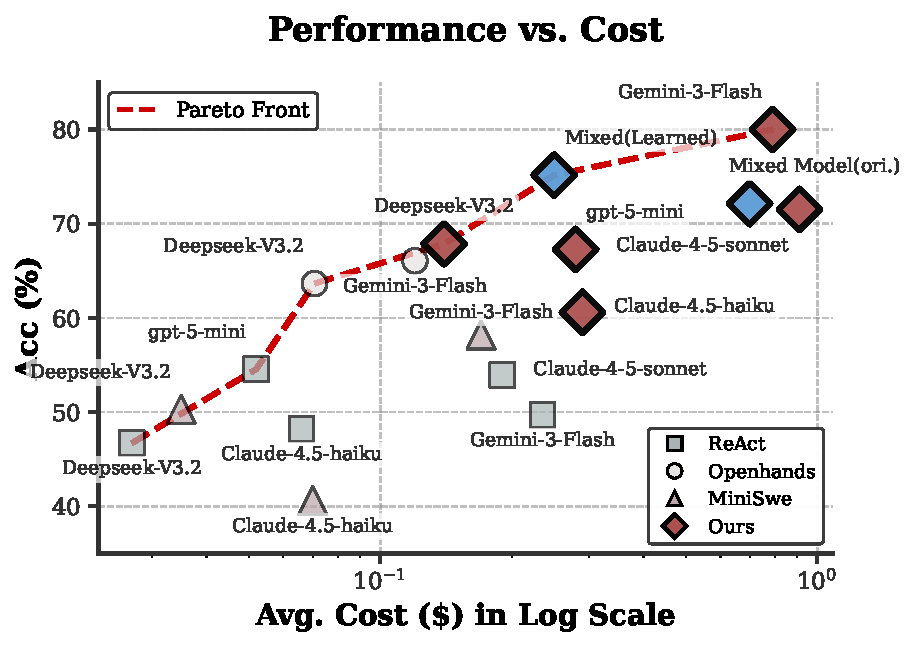
\includegraphics[width=\linewidth]{figures/gaia_cost_performance.pdf}
    \caption{\textbf{Pareto front curve of GAIA.} We plot GAIA accuracy and average cost per task (USD, log scale). Each point corresponds to a configuration, and the dashed curve indicates the Pareto frontier formed by \our across different model routing choices.}
    \label{fig:cost}
\end{figure}


\paragraph{In-context Learning for Cost-aware Orchestration}
Another advantage of \our{} is the ability to balance cost and performance through step-wise model routing.
Table~\ref{tab:level_main} shows that using different sub-agent models leads to markedly different accuracy--cost profiles, making it important for the orchestrator to be sensitive to such trade-offs.
We therefore apply a Pareto-oriented context learning procedure that iteratively optimizes the Orchestrator instruction from interaction trajectories with both performance and monetary cost feedback.
The resulting policy improves \our while reducing cost: under the mixed-model setting, Ours (ICL) improves accuracy from $72.12\%$ to $75.15\%$ while lowering average cost from \$0.70 to \$0.57 (Table~\ref{tab:level_main}), demonstrating that simple prompt-level learning can jointly enhance performance and efficiency.
At the system level, Figure~\ref{fig:cost} further shows that \our naturally yields strong Pareto-efficient operating points: across different model choices, our configurations form the Pareto frontier, indicating a systematically improved cost--performance trade-off over the baselines.


\subsubsection{Advantage 3: Plug-and-play Sub-agents}
\label{sec:adv3}
Here, we aim to verify the framework-level pluggability of our approach. 
Specifically, we replace the execution backend of the sub-agent with different agent frameworks, such as ReAct-style and Mini-SWE-style with \texttt{Gemini-3-Flash} as the orchestrator on Terminal-Bench, following the setups in Appendix~\ref{app:dataset}.

Table~\ref{tab:plugin_subagent} shows that when different sub-agent backends are used, \our maintains stable performance and consistently outperforms the corresponding baselines. 
This design allows sub-agents to be as pluggable modules, enabling the system to remain robust without depending on any particular sub-agent implementation.

\begin{table}[]
\centering
\setlength{\tabcolsep}{6pt}
\caption{Evaluating plug-and-play sub-agents with a fixed orchestrator. We use Gemini-3-Flash to test the robustness and reusability of different sub-agent implementations.
}
\label{tab:plugin_subagent}
\resizebox{\linewidth}{!}{%
\begin{tabular}{l c c c c}
\toprule
\textbf{System} 
& \textbf{Easy} 
& \textbf{Medium}
& \textbf{Hard} 
& \textbf{Acc} \\
\midrule

\multicolumn{5}{l}{\textbf{Standalone baselines}} \\
\midrule
ReAct                     & 50.00 & 34.09 & 16.67 & 28.57 \\
Mini-SWE-Agent            & 50.00 & 40.91& 20.83 & 34.29 \\
Claude Code               & 50.00 & 41.86 & 16.67 & 32.86 \\
\midrule

\multicolumn{5}{l}{\textbf{Orchestrator with plug-in sub-agents}} \\
\midrule
ReAct-style sub-Agent       & 50.00 & \textbf{63.63} & 20.83 & \textbf{48.57} \\
Mini-SWE-style sub-Agent   & \textbf{100.00} & 47.73 & \textbf{33.33} & 44.29 \\
\bottomrule
\end{tabular}
}
\end{table}

% \subsection{Case Study}
% \textcolor{red}{}
% We present the case study on GAIA. Please refer to Appendix~\ref{app:case_study}. 
%这里的